\name{df2}{two dimension digital filter}{digital filter}

\begin{synopsis}
 \item[df2] [ --f $f_0$ ] [ --p $f_1 \; b_1$ ] [ --z $f_2 \; b_2$ ] 
	    [ {\em infile} ]
 \end{synopsis}

 \begin{qsection}{DESCRIPTION}
 This command reads the input data file and passes it through a 2nd
  order digital filter. The central frequency and frequency band can
  be assigned through the options.
  The filter tranfer function is
  \[
   H(z)=\frac{1-2\exp(-\pi b_2/f_0)\cos(2\pi f_2/f_0)z^{-1} +
	\exp(-2\pi b_2/f_0)z^{-2}}
   {1-2\exp(-\pi b_1/f_0)\cos(2\pi f_1/f_0)z^{-1}+\exp(-2\pi b_1/f_0)z^{-2}}
  \]
 If this command is used in cascade, an arbitary filter can be
 designed using the options --p and --z.
 Input and output data are in float format.
 \end{qsection}

\begin{options}
	\argm{f}{f_0}{sampling frequency $f_0$ [Hz]}{10000}
	\argm{p}{f_1 \; b_1}{center frequency $f_1$ [Hz]
                and band width $b_1$ [Hz] of pole}{N/A}
	\argm{z}{f_2 \; b_2}{center frequency $f_2$ [Hz]
                and band width $b_2$ [Hz] of zero}{N/A}
\end{options} 

\begin{qsection}{EXAMPLE}
The command below gives impulse response of a filter with
a pole at 2000Hz and a frequency band of 200Hz:
\begin{quote}
 \verb!impulse | df2 -p 2000 200 !
\end{quote}
\hspace{3cm}
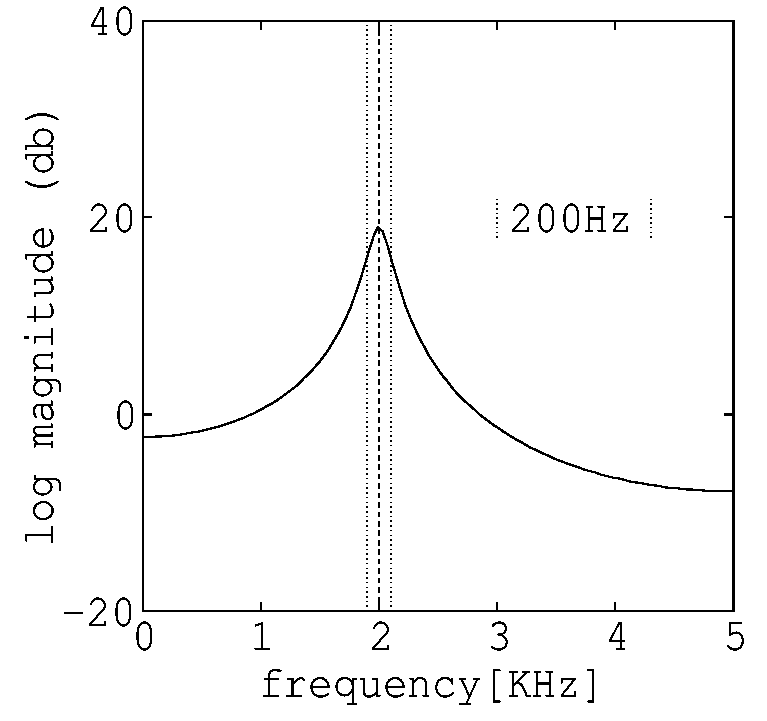
\includegraphics[width=4cm]{fig/df2.eps}
\end{qsection}
